\documentclass[mathserif]{beamer}

\setbeamertemplate{frametitle}[default][center]%Centers the frame title.
\setbeamertemplate{navigation symbols}{}%Removes navigation symbols.
\setbeamertemplate{footline}{\raisebox{5pt}{\makebox[\paperwidth]{\hfill\makebox[10pt]{\scriptsize\insertframenumber}}}}

\usepackage{amsmath,amssymb,amsthm,amsfonts}
\usepackage{nicefrac}
\usepackage{graphicx,array,dsfont}
\usepackage{wrapfig}
\usepackage{harvard}
\usepackage{multirow}
\citationmode{abbr}

\newcommand{\Hrule}{\rule{\linewidth}{0.2pt}}
\newcommand{\argmax}{\mathop{\mathrm{argmax}}}
\newcommand{\argmin}{\mathop{\mathrm{argmin}}}
\newcommand{\minimize}{\mathop{\mathrm{minimize}}}
\def\half{\frac{1}{2}}
\def\th{\mathrm{th}}
\def\sign{\mathrm{sign}}
\def\supp{\mathrm{supp}}
\def\E{\mathrm{E}}
\def\P{\mathrm{P}}
\def\Var{\mathrm{Var}}
\def\Cov{\mathrm{Cov}}
\def\Cor{\mathrm{Cor}}
\def\var{\mathrm{var}}
\def\cov{\mathrm{cov}}
\def\cor{\mathrm{cor}}
\def\rcor{\mathrm{rcor}}
\def\mcor{\mathrm{mcor}}
\def\mCor{\mathrm{mCor}}
\def\dCov{\mathrm{dCov}}
\def\dcov{\mathrm{dcov}}
\def\dVar{\mathrm{dVar}}
\def\dvar{\mathrm{dvar}}
\def\dCor{\mathrm{dCor}}
\def\dcor{\mathrm{dcor}}
\def\trace{\mathrm{trace}}
\def\col{\mathrm{col}}
\def\R{\mathds{R}} 
\def\cA{\mathcal{A}}
\def\cB{\mathcal{B}}
\def\cE{\mathcal{E}}
\def\cF{\mathcal{F}}
\def\cG{\mathcal{G}}
\def\cN{\mathcal{N}}
\def\hbeta{\hat{\beta}}
\def\hy{\hat{y}}
\def\red{\color[rgb]{0.8,0,0}}
\def\white{\color[rgb]{1,1,1}}
\def\blue{\color[rgb]{0,0,0.8}}
\def\green{\color[rgb]{0,0.4,0}}

\begin{document}

\title{Classification 3: Logistic regression (continued); 
model-free classification}
\author{Ryan Tibshirani \\ Data Mining: 36-462/36-662}
\date{April 9 2013}

\begin{frame}
\maketitle
{\it Optional reading: ISL 4.3, ESL 4.4; ESL 13.1--13.3}
\end{frame} 

\begin{frame}
\frametitle{Reminder: logistic regression}
\smallskip
Last lecture, we learned {\red logistic regression}, which
assumes that the log odds is linear in $x \in \R^p$:
$$\log\Big\{\frac{\P(C=1|X=x)}{\P(C=2|X=x)}\Big\}
= \beta_0+\beta^T x$$
This is equivalent to
$$\P(C=1|X=x) = \frac{\exp(\beta_0+\beta^Tx)}
{1+\exp(\beta_0+\beta^Tx)}$$
Given a sample $(x_i,y_i)$, $i=1,\ldots n$, we fit the coefficients 
by maximizing the log likelihood
$$\hbeta_0,\hbeta = \argmax_{\beta_0\in\R, \,\beta \in \R^p} \;
\sum_{i=1}^n \Big\{u_i \cdot (\beta_0+\beta^T x_i) -
\log\big(1+\exp(\beta_0+\beta^Tx_i)\big) \Big\}$$
where $u_i=1$ if $y_i=1$ and $u_i=0$ if $y_i=2$ (indicator for class 1)
\end{frame}

\begin{frame}
\frametitle{Classification by logistic regression}
\smallskip
\smallskip
After computing $\hbeta_0,\hbeta$, {\red classification} of an input 
$x\in\R^p$  is given by
$$\hat{f}^{\mathrm{LR}}(x) = \begin{cases}
1 & \mathrm{if} \; \hbeta_0+\hbeta^T x > 0 \\
2 & \mathrm{if} \; \hbeta_0+\hbeta^T x \leq 0 \\
\end{cases}$$
Why? Recall that the log odds between class 1 and class 2 is modeled as
$$\log\Big\{\frac{\P(C=1|X=x)}{\P(C=2|X=x)}\Big\} 
= \beta_0+\beta^T x$$

\smallskip
Therefore the {\red decision boundary} between classes 1 and 2 is the set of 
all $x \in \R^p$ such that
$$\hbeta_0+\hbeta^T x = 0$$
This is a $(p-1)$-dimensional affine subspace of $\R^p$; i.e., this is a point
(threshold) in $\R^1$, or a line in $\R^2$
\end{frame}

\begin{frame}
\frametitle{Interpretation of logistic regression coefficients}
\smallskip
How do we interpret coefficients in a logistic regression? Similar
to our interpretation for linear regression. Let 
$$\Omega = \log\Big\{\frac{\P(C=1|X=x)}{\P(C=2|X=x)}\Big\}$$ be the log odds. 
Then logistic regression provides the estimate
$$\hat{\Omega} \;=\; \hbeta^T x \;=\; 
\hbeta_0+\hbeta_1x_1 + \hbeta_2 x_2 + \ldots +\hbeta_p x_p$$
Hence, the proper {\red interpretation} of $\hbeta_j$: increasing the $j$th 
predictor $x_j$ by 1 unit, and keeping all other predictors fixed, increases
\begin{itemize} 
\item The estimated log odds of class 1 by an additive factor of $\hbeta_j$
\item The estimated odds of class 1 by a multiplicative factor of $e^{\hbeta_j}$
\end{itemize}
\smallskip
\smallskip
(Note: it may not always be possible for a 
predictor $x_j$ to increase with the other predictors fixed!)
\end{frame}

\begin{frame}
\frametitle{Example: South African heart disease data}
Example (from ESL section 4.4.2): there are $n=462$ individuals broken up
into 160 {\red cases} (those who have coronary heart disease) and 
302 {\red controls} (those who don't). There are $p=7$ variables measured on
each individual:

\bigskip
\begin{itemize}
\item sbp (systolic blood pressure) 
\item tobacco (lifetime tobacco consumption in kg) 
\item ldl (low density lipoprotein cholesterol) 
\item famhist (family history of heart disease, present or absent) 
\item obesity 
\item alcohol 
\item age 
\end{itemize}
\end{frame}

\begin{frame}
\frametitle{}
\bigskip
Pairs plot (red are cases, green are controls):
\begin{center}
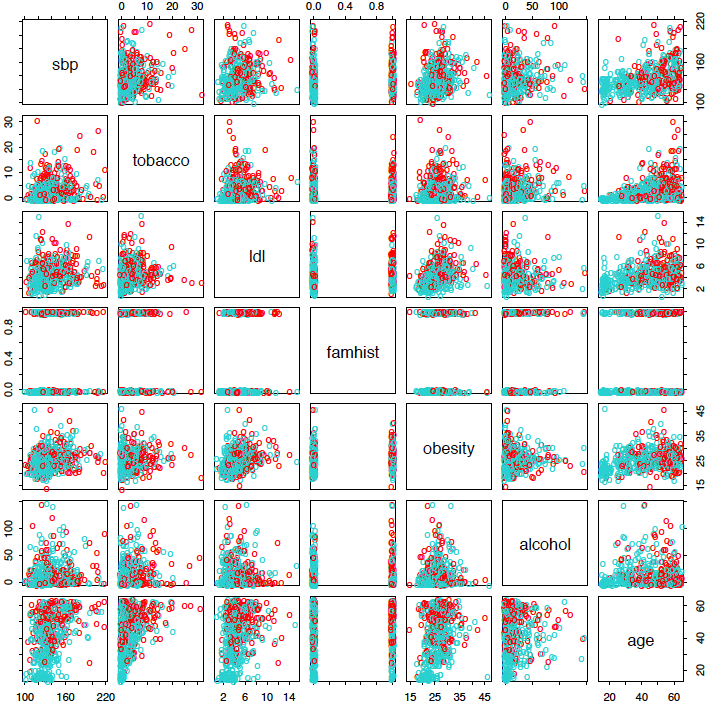
\includegraphics[width=2.75in]{sapairs.png}
\end{center}
\end{frame}

\begin{frame}
\frametitle{}
\smallskip
\smallskip
Fitted logistic regression model:
\begin{center}
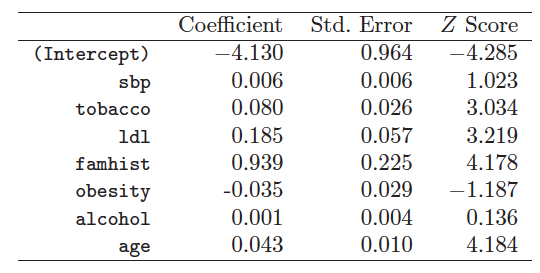
\includegraphics[width=2.75in]{salr1.png}
\end{center}
The $Z$ score is the coefficient divided by its standard error. 
There is a test for significance called the Wald test

\bigskip
Just as in linear regression, {\red correlated variables} can cause problems with
interpretation. E.g.,
sbp and obseity are not significant, and obesity has a negative sign! (Marginally, 
these are both significant and have positive signs) 
\end{frame}

\begin{frame}
\frametitle{}
\bigskip
After repeatedly dropping the least significant variable and refitting:
\begin{center}
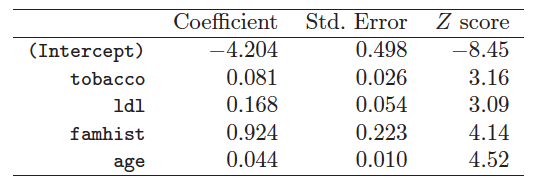
\includegraphics[width=2.75in]{salr2.png}
\end{center}
This procedure was stopped when all variables were significant

\bigskip
E.g., interpretation of tobacco coefficient: increasing the tobacco 
usage over the course of one's lifetime by 1kg (and keeping all other 
variables fixed) multiplies the estimated odds of coronary heart 
disease by $\exp(0.081) \approx 1.084$, or in other words, increases 
the odds by $8.4\%$
\end{frame}

\begin{frame}
\frametitle{LDA versus logistic regression}
As we remarked earlier, both LDA and logistic regression model the log
odds as a linear function of the predictors $x \in \R^p$
\begin{align*}
\text{Linear discriminant analysis:} \;\;
&\log\Big\{\frac{\P(C=1|X=x)}{\P(C=2|X=x)}\Big\}
= \alpha_0+\alpha^T x \\
\text{Logistic regression:} \;\;
& \log\Big\{\frac{\P(C=1|X=x)}{\P(C=2|X=x)}\Big\}
= \beta_0+\beta^T x
\end{align*}
where for LDA we form $\hat{\alpha}_0,\hat{\alpha}$ based on 
estimates $\hat{\pi}_j,\hat{\mu}_j,\hat{\Sigma}$
(easy!), and for logistic regression we estimate 
$\hbeta_0,\hbeta$ directly based on maximum likelihood (harder)

\bigskip
This is what leads to linear decision boundaries for each method

\bigskip
Careful inspection (or simply comparing them in R) shows that the 
estimates $\hat{\alpha}_0,\hbeta_0$ and $\hat{\alpha},\hbeta$
are {\red different}. So how do they compare?
\end{frame}

\begin{frame}
\frametitle{}
\smallskip
\smallskip
Generally speaking, logistic regression is more flexible because it doesn't assume
anything about the distribution of $X$. LDA assumes that $X$ is normally distributed 
within each class, so that its marginal distribution is a mixture of normal distributions, 
hence still normal:
$$X \sim \sum_{j=1}^K \pi_j N(\mu_j,\Sigma)$$
This means that logistic regression is {\red more robust} to situations in which the 
class conditional densities are not normal (and outliers

\bigskip
On the other side, if the true class conditional densities are normal, or close to it, LDA will be
{\red more efficient}, meaning that for logistic regression to perform comparably it will need more data

\bigskip
In practice they tend to perform similarly in a variety of situations (as claimed by the ESL book on page
128)
\end{frame}

\begin{frame}
\frametitle{Extensions}
Logistic regression can be adapted for {\red multiple classes}, $K>2$. We model
the log odds of each class to a base class, say, the last one:
\vspace{-1pt}
$$\log\Big\{\frac{\P(C=j|X=x)}{\P(C=K|X=x)}\Big\}
= \beta_{0,j}+\beta_j^T x
\vspace{-1pt}$$
We fit the coefficients, $j=1,\ldots K$, jointly by maximum likelihood

\bigskip
For {\red high-dimensional problems} with $p>n$, we run into problems with LDA
in estimating the $p \times p$ covariance matrix $\Sigma$: with only $n$ observations, out 
estimate $\hat{\Sigma}$ will not be invertible. {\red Regularized LDA} remedies this by 
shrinking $\hat{\Sigma}$ towards the identity, using the estimate
$c\cdot\hat{\Sigma} + (1-c)\cdot I$ for some $0<c<1$

\bigskip
For regularization in logistic regression, we can subtract a {\red penalty}, e.g., 
an $\ell_1$ penalty: $\lambda \|\beta\|_1$,
from the maximum likelihood criterion, similar to what we
did in linear regression
\end{frame}

\begin{frame}
\frametitle{Model-free classification}
It is possible to perform classification in a {\red model-free} sense, i.e.,
without writing down any assumptions concerning the distribution that generated the data

\bigskip
The downside: these methods are essentially a {\red black box} for classification, in
that they typically don't provide any insight into how the predictors and the response
are related

\bigskip
The upside: they can work well for prediction in a wide variety of situations, since they
don't make any real assumptions

\bigskip
These procedures also typically have {\red tuning parameters} that need to be properly
tuned in order for them to work well (for this we can use cross-validation)
\end{frame}

\begin{frame}
\frametitle{Classification by $k$-nearest-neighbors}
Perhaps the simplest prediction rule, given labeled data $(x_i,y_i)$, $i=1\ldots n$, 
is to predict an input $x \in \R^p$ according to its {\red nearest- neighbor}:
$$\hat{f}^{1-\mathrm{NN}}(x) = y_i \;\;\; \mathrm{such}\;\mathrm{that} \;\|x_i-x\|_2
\;\mathrm{is}\;\mathrm{smallest}$$

\smallskip
A natural extension is to consider the {\red $k$-nearest-neighbors} of $x$, call
them $x_{(1)},\ldots x_{(k)}$, and then classify according to a majority vote:
$$\hat{f}^{k-\mathrm{NN}}(x) = j \;\;\; \mathrm{such}\;\mathrm{that} \;
\sum_{i=1}^k 1\{y_{(i)}=j\} \;\;\mathrm{is}\;\mathrm{largest}$$

\smallskip
What is more adaptive, 1-nearest-neighbor or 9-nearest-neighbors? What is the
$n$-nearest-neighbors rule?
\end{frame}

\begin{frame}
\frametitle{Example: 7-nearest-neighbors classifier}
\smallskip
\smallskip
Example: classification with 7-nearest-neighbors (ESL page 467):
\begin{center}
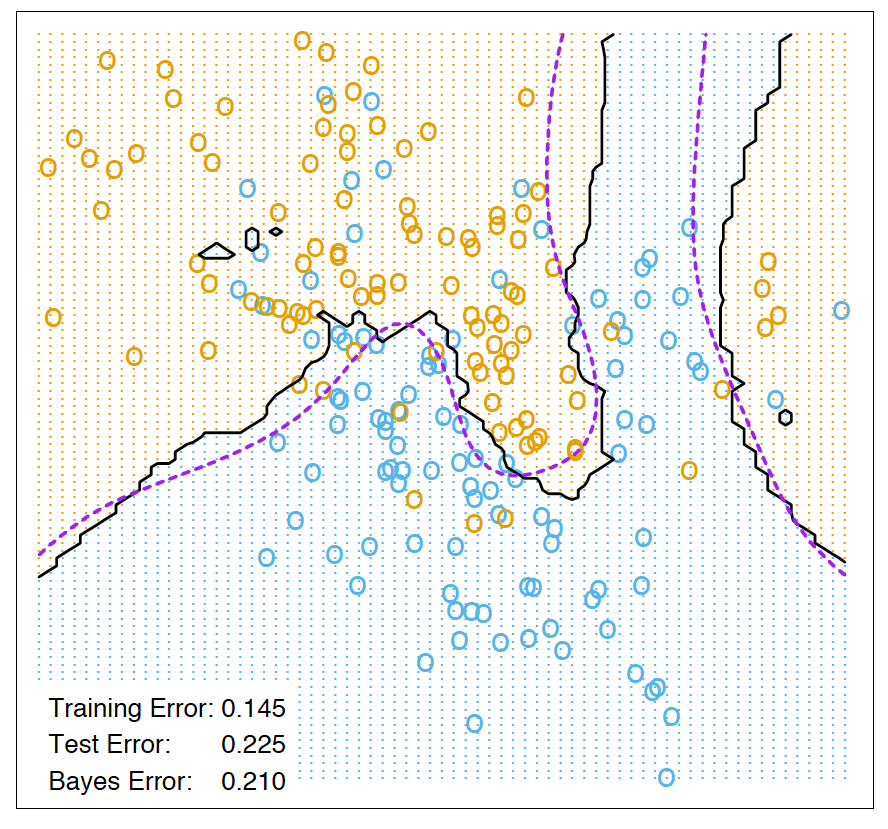
\includegraphics[width=2.5in]{7nn.png}
\end{center}
Could linear discriminant analysis or logistic regression have drawn decision 
boundaries close to the Bayes boundary? 
\end{frame}

\begin{frame}
\frametitle{Disadvantages of $k$-nearest-neighbors}
Besides the fact that it yields {\red limited insight} into the relationship 
between the predictors
and classes, there are disadvantages of using a $k$-nearest-neighbors rule having
to do with {\red computation}

\bigskip
For one, we need the {\red entire data set} $(x_i,y_i)$, $i=1,\ldots n$ 
whenever we want to classify a new point $x \in \R^p$. This could end
up being very prohibitive, especially if $n$ and/or $p$ are large. 
On the other hand, for prediction with LDA or logistic regression, we only need
the linear coefficients that go into the prediction rule

\bigskip
Even with the entire data set at hand, the prediction rule is {\red slow}. It essentially
requires comparing distances to every point in the training set. There are somewhat 
fancy ways of storing the data to make this happen as fast a possible, but they're 
still pretty slow
\end{frame}

\begin{frame}
\frametitle{Classification by $K$-means clustering}
Instead of using every point in the data set $(x_i,y_i)$, $i=1,\ldots n$, we can
try to {\red summarize} this data set, and use this for classification

\bigskip
How would we do this? We've covered many unsupervised learning techniques; one of 
the first was {\red $K$-means clustering}. Consider the following procedure 
for classification:
\smallskip
\begin{itemize}
\item Use $R$-means clustering to fit $R$ centroids $c_1(j),\ldots c_R(j)$ 
separately to the data within each class $j=1,\ldots K$;
\item Given an input $x \in \R^p$, classify according to the class of the nearest
centroid:
\begin{align*}
\hat{f}^{R-\mathrm{means}}(x) = j \;\;\;&\mathrm{such}\;\mathrm{that}\;
\|x-c_i(j)\|\;\mathrm{is}\;\mathrm{smallest}\\
&\;\mathrm{for}\;\mathrm{some}\;i=1,\ldots R
\end{align*}
\end{itemize}

We only need the $K\cdot R$ centroids $c_1(j),\ldots c_K(j)$, 
$j=1,\ldots K$ for classification
\end{frame}

\begin{frame}
\frametitle{Example: 5-means clustering for classification}
\smallskip
\smallskip
Example: same data set as before, now we use 5-means clustering within
each class, and classify according to the closest centroid (from ESL page 464):
\begin{center}
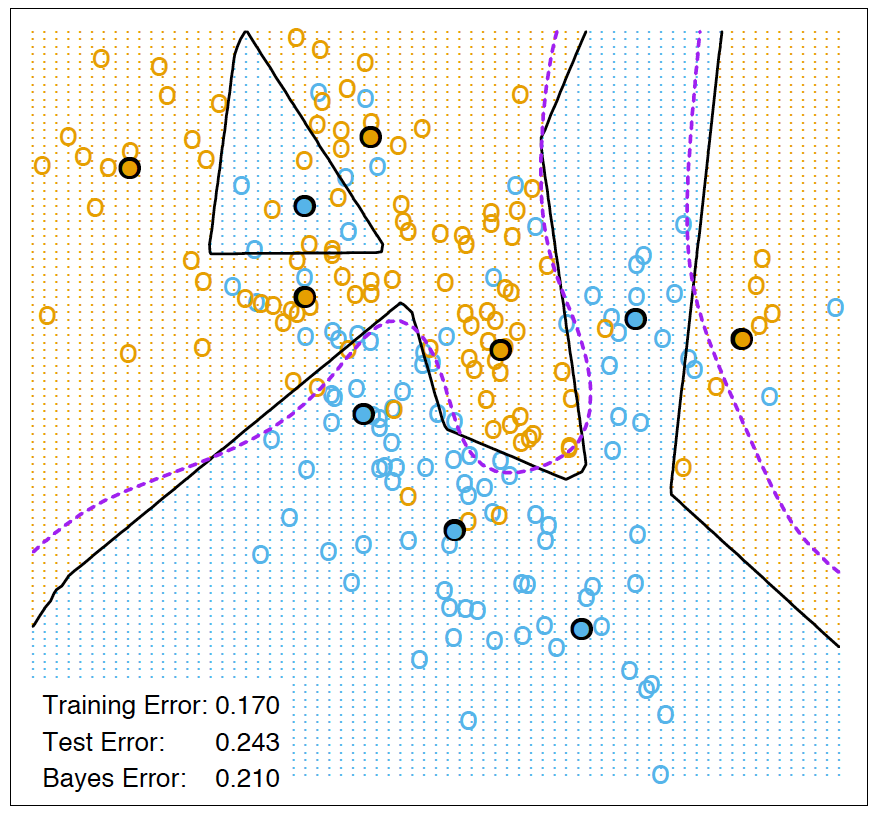
\includegraphics[width=2.5in]{5m.png}
\end{center}
\end{frame}

\begin{frame}
\frametitle{Learning vector quantization}
One downside of $K$-means clustering used in this context is that, for each 
class, the centroids are chosen without any say from other classes. This can
result in centroids being chosen close to decision boundaries, which is bad

\bigskip
{\red Learning vector quantization}\footnote{Kohonen (1989), ``Self-Organization
and Associative Memory''} takes
this into consideration, and places $R$ prototypes for each class 
strategically away from decision boundaries. Once these prototypes have been
chosen, classification proceeds in the same way as before (according to the
class of the nearest prototype)

\bigskip
Given $(x_i,y_i)$, $i=1,\ldots n$, learning vector quantization
chooses the prototypes as follows:
\begin{itemize}
\item[1.] Choose $R$ initial protoypes $c_1(j),\ldots c_R(j)$ for
$j=1,\ldots K$ (e.g., sample $R$ training points at random for each class)
\end{itemize}
\end{frame}

\begin{frame}
\frametitle{}
\smallskip
\begin{itemize}
\item[2.] Choose a training point $x_\ell$ at random. Let $c_i(j)$ be the closest
protoype to $x_\ell$. If:
\begin{itemize}
\item[(a)] $y_\ell=j$, then move $c_i(j)$ closer to $x_\ell$:
$$c_i(j) \leftarrow c_i(j) + \epsilon(x_\ell-c_i(j))$$
\item[(b)] $y_\ell\not=j$, then move $c_i(j)$ away from $x_\ell$:
$$c_i(j) \leftarrow c_i(j) - \epsilon(x_\ell-c_i(j))$$
\end{itemize}
\item[3.] Repeat step 2, decreasing $\epsilon \rightarrow 0$ with each iteration
\end{itemize}

\bigskip
The quantity $\epsilon \in (0,1)$ above is called the ``learning rate''. It 
can be taken, e.g., as $\epsilon=1/r$, where $r$ is the iteration number

\bigskip
Learning vector quantization can sometimes perform better than classification
by $K$-means clustering, but other times they perform {\red very similarly}
(e.g., in the previous example)
\end{frame}

\begin{frame}
\frametitle{Tuning parameters}
Each one of these methods exhbitis a {\red tuning parameter} that needs
to be chosen. E.g.,
\begin{itemize}
\item the number $k$ of neighbors in $k$-nearest-neighbors
\item the number $R$ of centroids in $R$-means clustering
\item the number $R$ of prototypes in learning vector quantization
\end{itemize}

\bigskip
Think about the bias-variance tradeoff at play here---for each 
method, which direction means higher model complexity?

\bigskip
As before, a good method for choosing tuning parameter
values is {\red cross-validation}, granted that we're looking to 
minimize prediction error
\end{frame}

\begin{frame}
\frametitle{Example: cross-validation for $k$-nearest-neighbors}
\smallskip\smallskip
Example: choosing the number of neighbors $k$ using 10-fold cross-
validation (from ESL page 467):

\begin{center}
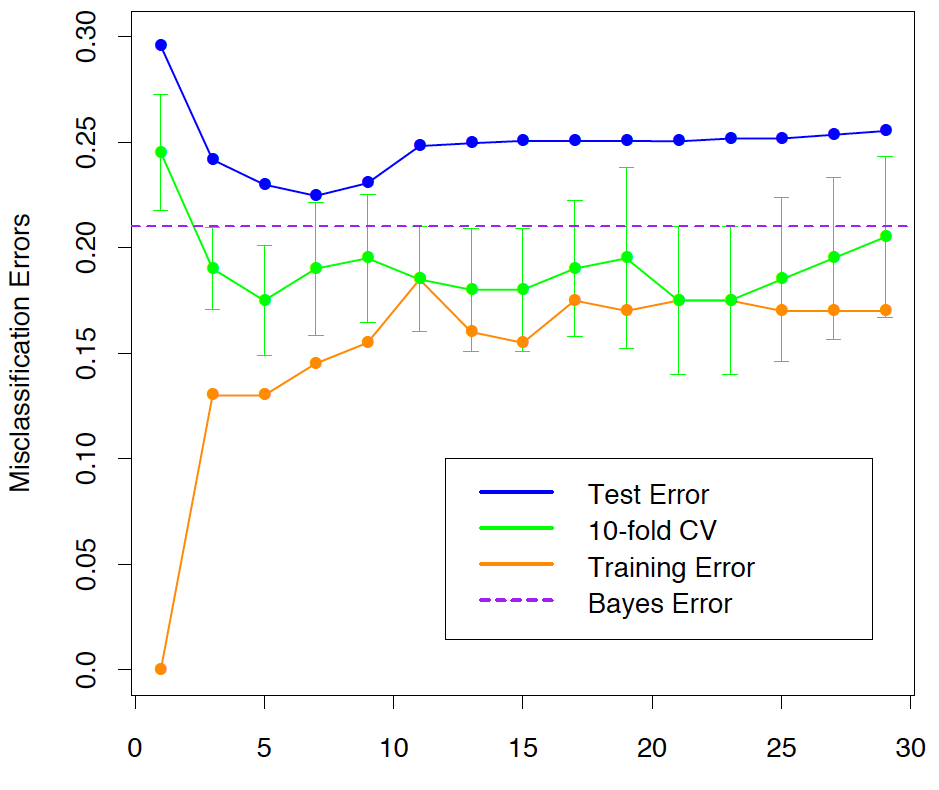
\includegraphics[width=2.75in]{tune.png}
\end{center}
\end{frame}

\begin{frame}
\frametitle{Classification tools in R}
\smallskip\smallskip
The classification tools we've learned so far, in R:

\smallskip
\begin{itemize}
\item Linear discriminant analysis: use the {\tt lda} function
in the {\tt MASS} package. For reduced-rank LDA of dimension $L$,
take the first $L$ columns of the {\tt scaling} matrix

\smallskip
\item Logistic regression: use the {\tt glm} function in the base package. 
It takes the same syntax as the {\tt lm} function; make sure to set
{\tt family="binomial"}. Can also apply regularization using {\tt glmnet}

\smallskip
\item $k$-nearest-neighbors: use the {\tt knn} function in the 
{\tt class} package

\smallskip
\item $K$-means clustering: use the {\tt kmeans} function in the
{\tt stats} package for the clustering; classification to the nearest
centroid can then be done manually

\smallskip
\item Learning vector quantization: use the {\tt lvq1} function in
the {\tt class} package. Here the list of protoypes is called the 
``codebook'' and passed as the {\tt codebk} argument
\end{itemize}
\end{frame}

\begin{frame}
\frametitle{Recap: logistic regression, model-free classification}
\smallskip
In this lecture, we learned more about {\red logistic regression}.
We saw that is draws linear decision boundaries between the classes
(linear in the predictor variable $x \in \R^p$), and learned how
to interpret the coefficients, in terms of a multiplicative change
in the odds ratio

\bigskip
We also {\red compared} logistic regression and LDA. Essentially,
logistic regression is more robust because it doesn't assume normality,
and LDA performs better if the normal assumption is (close to) true

\bigskip
We learned several {\red model-free} classification techniques. 
Typically these don't help with understanding the relationship between
the predictors and the classes, but they can perform well in terms of 
prediction error. 
The {\red $k$-nearest-neighbors} method classifies a new input by looking at 
its $k$ closest neighbors in the training set, and then classifying 
according to a majority vote among their labels. {\red $K$-means
clustering} and {\red learning vector quantization} represent each class 
by a number of centroids or prototypes, and then use these to classify, 
and so they are more computationally efficient
\end{frame}

\begin{frame}
\frametitle{Next time: tree-based methods}
Classification trees are popular because they are easy to interpret

\smallskip
\begin{center}
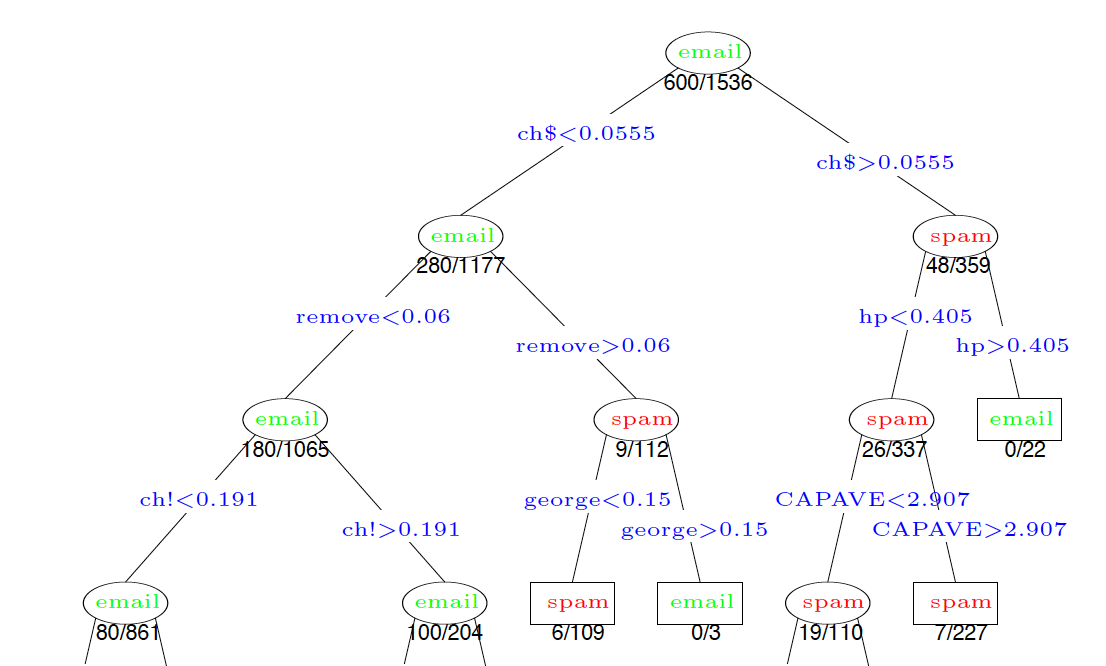
\includegraphics[width=3.25in]{tree.png}
\end{center}

\bigskip
(From ESL page 315)
\end{frame}
\end{document}


